% Exam Template for San Jacinto Community College Math Department courses
%Copyright@Chandi Bhandari
%%%%%%%%%%%%%%%%%%%%%%%%%%%%%%%%%%%%%%%%%%%%%%%%%%%%%%%%%%%%%%%%%%%%%%%%%%%%%%%%%%%%%%%%%%%%%%

% These lines can probably stay unchanged, although you can remove the last
% two packages if you're not making pictures with tikz.
\documentclass[11pt]{exam}
\RequirePackage{amssymb, amsfonts, amsmath, latexsym, verbatim, xspace, setspace}
\RequirePackage{tikz, pgflibraryplotmarks}
\usepackage{graphicx}
\graphicspath{ {./images/} }

% By default LaTeX uses large margins.  This doesn't work well on exams; problems
% end up in the "middle" of the page, reducing the amount of space for students
% to work on them.
\usepackage[margin=1in]{geometry}


% Here's where you edit the Class, Exam, Date, etc.
\newcommand{\class}{Math 2412 Pre-Calculus}
\newcommand{\term}{Summer 2018}
\newcommand{\examnum}{Exam III}
\newcommand{\examdate}{July, 2018}
\newcommand{\timelimit}{90 Minutes}

% For an exam, single spacing is most appropriate
\singlespacing
% \onehalfspacing
% \doublespacing

% For an exam, we generally want to turn off paragraph indentation
\parindent 0ex

\begin{document} 

% These commands set up the running header on the top of the exam pages
\pagestyle{head}
\firstpageheader{}{}{}
\runningheader{\class}{\examnum\ - Page \thepage\ of \numpages}{\examdate}
\runningheadrule

\begin{flushright}
\begin{tabular}{p{3.2in} r l}
\textbf{\class} & \textbf{\term} & \textbf{\examnum}\\
\textbf{G-Number-} & \textbf{Name (Print):}  \makebox[1.2in]{\hrulefill}\\
%\textbf{Time: \timelimit} % & \makebox[2in]{\hrulefill}

\end{tabular}\\
\end{flushright}
\rule[1ex]{\textwidth}{.1pt}

%\bf{ Choose Any 10 questions}

\hfill


%%%%%%%%%%%%%%%%%%%%%%%%%%%%%%%%%%%%%%%%%%%%%%%%%%%%%%%%%%%%%%%%%%%%%%%%%%%%%%%%%%%%%
%For the further information 
%%%%%%%%%%%%%%%%%%%%%%%%%%%%%%%%%%%%%%%%%%%%%%%%%%%%%%%%%%%%%%%%%%%%%%%%%%%%%%%%%%%%%

\begin{questions}

% Basic question
\addpoints
\question[10] Simplify 
\begin{parts}
\part[3] Solve the equation
\begin{align*}
e^{2x}-3e^x+2=0
\end{align*}
\vspace{7cm}
\part[3] Solve the equation
\begin{align*}
log(x) + log(x-1)=log(4x)
\end{align*}
\vspace{7cm}
\part[4] Find the reference angle and 3 coterminal angles (with at least one negative) for $210^\circ$ .
\end{parts}
\vspace{8cm}
% Question with parts
%\newpage
\addpoints
\question[3]Find the sector for the given figure. 
\begin{center}
	\includegraphics{sectorarea.png}
\end{center}
\addpoints
\question[10] Find the value of the following
\begin{parts}
\part[2] $cos(\frac{\pi}{6})$
\vspace{1cm}
\part[2]  $cot(-\frac{\pi}{3})$
\vspace{1cm}
\part[2] $sin(\frac{5\pi}{4})$
\vspace{1cm}.
\part[2]  $cot(120^\circ)$
\vspace{1cm}
\part[2] $tan(-60^\circ)$
\vspace{1cm}
\end{parts}

\newpage
\vspace{8cm}
\addpoints
\question[10] A certain species of bird was introduced in a certain county 25 years ago. Biologist observer that the population doubles every 10 years, and now the population is 13,000.   
\begin{parts}
\part What was the initial size of the bird population?
\part Estimate the bird population 5 years from now. 
\end{parts}

\vspace{9cm}
\addpoints
\question[10] Draw the graph by making the table of  $f(x)=cos^{-1}(x)$. Also, State its domain and range.
	\begin{center}
	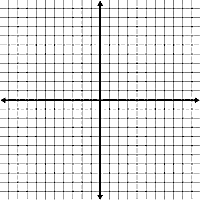
\includegraphics{graph1.png}	
	\end{center}

\newpage
\addpoints
\question[10] Find the Domain, rage, period, Horizontal and Vertical, amplitude shift of the following function and  graph one period of $f(x)=2sin(2x+\frac{\pi}{4})+5$

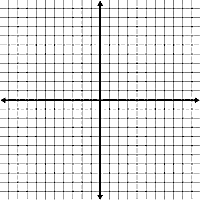
\includegraphics{graph1.png}
\vspace{9cm}
\addpoints
\question[10] Graph the one period of $y=3tan(x-\frac{\pi}{4})$







\vspace{8cm}
\addpoints
\question[7] From the top of the 200-ft lighthouse, the angle of depression to a ship in the ocean is $30^\circ$. How far is the ship from the base of lighthouse?


\vspace{9cm}
\addpoints
\question[10] Find the measure of all angles $\angle A, \angle B$ and, $\angle C$ for the following graph.
\begin{center}
	\includegraphics{cosruletr.png}
\end{center}


\vspace{8cm}
\noaddpoints
\question[10] Find all the missing parts of the triangle. Round all angles to the nearest hundredth of a degree and all sides to the hundredth of a unit.
\begin{center}
	\includegraphics{sinruletr.png}
\end{center}
 
\vspace{8cm}
\noaddpoints
\question[10] 
\begin{parts}
	\part [5] Write down $tan(\theta)$ in terms of $cos(\theta)$ in the II quadrant. 
	\vspace{8cm}
	\part [5] Find the all angle and sides. 
\begin{center}
	\includegraphics{pythagoreantr.png}
\end{center}
\end{parts}
\vspace{8cm}
\noaddpoints
\question[5 Bonus] Find the exact value of $cos^{-1}(tan(sin^{-1}(\frac{\sqrt{2}}{2})))$
\end{questions}
\end{document}